\documentclass{config}
\usepackage[T1]{fontenc}
\usepackage[utf8]{inputenc}
\usepackage{graphicx}
\usepackage{color}
\usepackage{siunitx}
\usepackage{listings}
\usepackage{wrapfig}
\usepackage{subcaption}
\usepackage{float}
\usepackage[toc,page]{appendix} 
\usepackage{amsmath}
\usepackage{bigints}
\usepackage{multicol}
\newcommand\x{\XSolid}

\usepackage[labelfont=sc]{caption}
\title{Clamping}
%\author{Jeanne VENTRE}

%\instlabel{}{Master 2 of Engineering in Fluid Mechanics Fundamentals and Applications, Pierre and Marie Curie University (UPMC)}

\begin{document}

\maketitle

\begin{figure}[H]
\begin{center}
\includegraphics[scale=0.48]{Clamping.png}
\caption{}
\label{schema}
\end{center}
\end{figure}

\begin{table}[H]
\begin{center}
\begin{tabular}{|c|c|c|}
\hline
 & Pré-clamp & Post-clamp \\ 
\hline 
Total resistance & 41.8 g.s$^{-1}$.cm$^{-4}$ & 67.2 g.s$^{-1}$.cm$^{-4}$ \\
\hline
\hline 
Ratio pre/post & \multicolumn{2}{|c|}{0.62}\\
\hline
\end{tabular} 
\caption{Theoretical calculation of total resistance.}
\label{res_pré}
\end{center}
\end{table}



\begin{figure}[H]
\centering
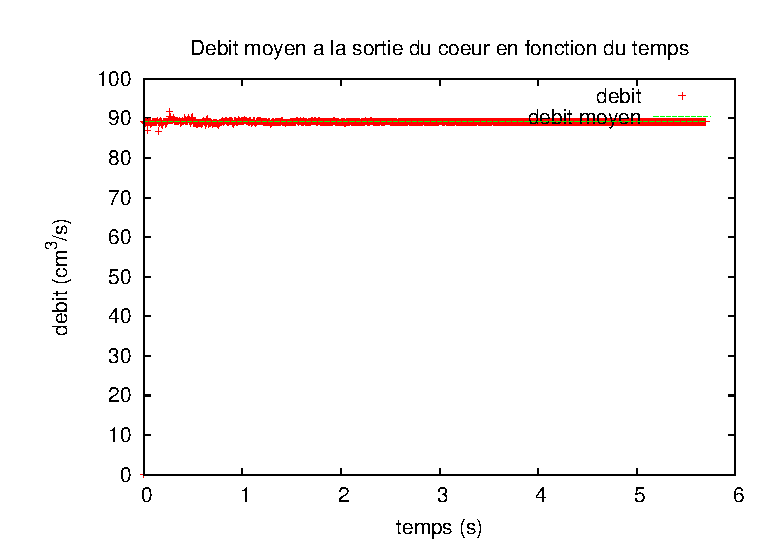
\includegraphics[scale=1]{Q.eps}
\caption{Débit d'entrée mesuré à la sortie du coeur.}
\label{debit_entree}
\end{figure}

\begin{figure}[H]
\begin{minipage}{.48\textwidth}
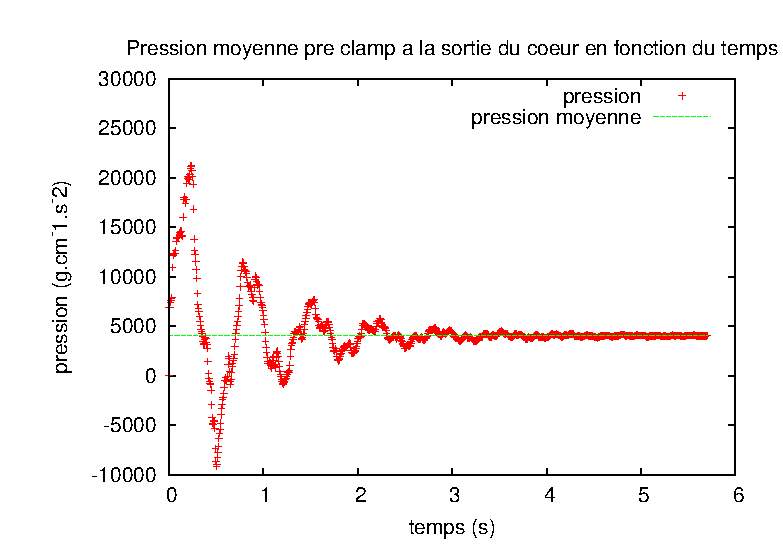
\includegraphics[scale=0.7]{preclampP.eps}
\end{minipage} \hfill
\begin{minipage}{.48\textwidth}
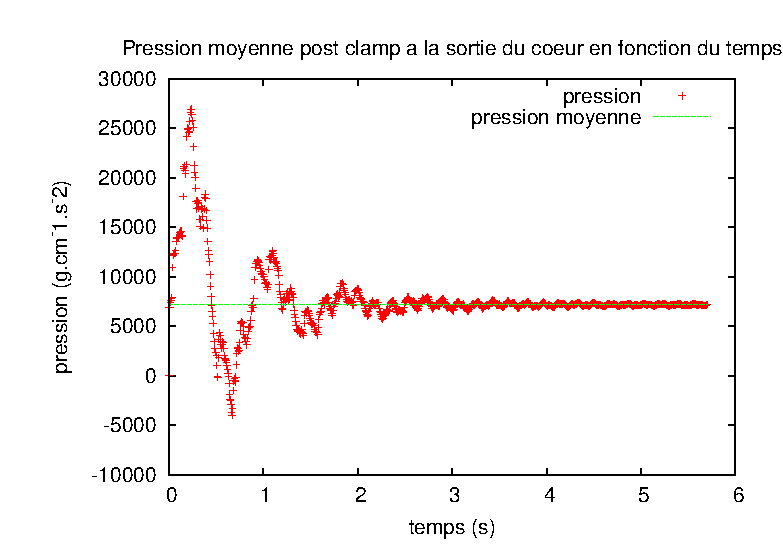
\includegraphics[scale=0.7]{postclampP.eps}
\end{minipage}
\caption{Pression à la sortie du coeur. \`A gauche : pré clamp, à droite : post clamp}
\end{figure}

\begin{table}[H]
\begin{center}
\begin{tabular}{|c|c|c|}
\hline
 & Pré-clamp & Post-clamp \\ 
\hline 
Résistance totale & 45.5 g.s$^{-1}$.cm$^{-4}$ & 80.8 g.s$^{-1}$.cm$^{-4}$ \\
\hline
\hline 
Ratio pre/post & \multicolumn{2}{|c|}{0.56}\\
\hline
\hline 
Erreur & $\sim  8 \%$  & $\sim 20 \%$ \\ 
\hline
\end{tabular} 
\caption{Calcul numérique des résistances }
\label{res_post}
\end{center}
\end{table}



\end{document}
